\documentclass[11pt,a4paper,twoside,openright]{report}

\usepackage[top=25mm,bottom=25mm,right=25mm,left=30mm,head=12.5mm,foot=12.5mm]{geometry}
\let\openright=\cleardoublepage

\usepackage[a-2u]{pdfx}

\usepackage[
   backend=biber
%  ,style=iso-authoryear
  ,style=alphabetic
  ,citestyle=numeric
  ,sortlocale=cs_CZ
  ,bibencoding=UTF8
  %,block=ragged
]{biblatex}
\addbibresource{references.bib}

%% Přepneme na českou sazbu, fonty Latin Modern a kódování češtiny
\usepackage[czech]{babel}
\usepackage{lmodern}
\usepackage[T1]{fontenc}
\usepackage{textcomp}
\usepackage[utf8]{inputenc}

\usepackage{subcaption}


\begin{comment}
% Set fonts
\RequirePackage[osf]{mathpazo} % Palatino with oldstyle figures
\newcommand\liningnums[1]{\fontfamily{ppl}\selectfont#1}
\RequirePackage{eulervm}
\RequirePackage[scaled=.8819]{sourcecodepro} % Source Code Pro typeface for monospace
\end{comment}

%%% Další užitečné balíčky (jsou součástí běžných distribucí LaTeXu)
\usepackage{amsmath}        % rozšíření pro sazbu matematiky
\usepackage{amsfonts}       % matematické fonty
\usepackage{amsthm}         % sazba vět, definic apod.
\usepackage{bm}             % tučné symboly (příkaz \bm)
\usepackage{graphicx}       % vkládání obrázků
\usepackage{fancyvrb}       % vylepšené prostředí pro strojové písmo
\usepackage{fancyhdr}       % prostředí pohodlnější nastavení hlavy a paty stránek
\usepackage{icomma}         % inteligetní čárka v matematickém módu
\usepackage{dcolumn}        % lepší zarovnání sloupců v tabulkách
\usepackage{booktabs}       % lepší vodorovné linky v tabulkách
\makeatletter
\@ifpackageloaded{xcolor}{
   \@ifpackagewith{xcolor}{usenames}{}{\PassOptionsToPackage{usenames}{xcolor}}
  }{\usepackage[usenames]{xcolor}} % barevná sazba
\makeatother
\usepackage{multicol}       % práce s více sloupci na stránce
\usepackage{caption}
\usepackage{enumitem}
\usepackage{lipsum}
\setlist[itemize]{noitemsep, topsep=0pt, partopsep=0pt}
\setlist[enumerate]{noitemsep, topsep=0pt, partopsep=0pt}
\setlist[description]{noitemsep, topsep=0pt, partopsep=0pt}
\usepackage{pdfpages}

\usepackage{tocloft}
\setlength\cftparskip{0pt}
\setlength\cftbeforechapskip{1.5ex}
\setlength\cftfigindent{0pt}
\setlength\cfttabindent{0pt}
\setlength\cftbeforeloftitleskip{0pt}
\setlength\cftbeforelottitleskip{0pt}
\setlength\cftbeforetoctitleskip{0pt}
\renewcommand{\cftlottitlefont}{\Huge\bfseries}
\renewcommand{\cftloftitlefont}{\Huge\bfseries}
\renewcommand{\cfttoctitlefont}{\Huge\bfseries}

% vyznaceni odstavcu
\parindent=0pt
\parskip=11pt

% zakaz vdov a sirotku - jednoradkovych pocatku ci koncu odstavcu na prechodu mezi strankami
\clubpenalty=1000
\widowpenalty=1000
\displaywidowpenalty=1000

% nastaveni radkovani
\renewcommand{\baselinestretch}{1.20}

% nastavení hlavy a paty stránek
\fancyhf{}
\renewcommand{\chaptermark}[1]{\markboth{#1}{}}
\fancyhead[RO,LE]{\leftmark}
\fancyfoot[RO,LE]{\thepage}
%\renewcommand{\footrulewidth}{0pt}
\fancypagestyle{plain}{%
\fancyhf{} % clear all header and footer fields
\fancyfoot[RO,LE]{\thepage}
\renewcommand{\headrulewidth}{0pt}
%\renewcommand{\footrulewidth}{0.5pt}
}

% Tato makra přesvědčují mírně ošklivým trikem LaTeX, aby hlavičky kapitol
% sázel příčetněji a nevynechával nad nimi spoustu místa. Směle ignorujte.
\makeatletter
\def\@makechapterhead#1{
  {\parindent \z@ \raggedright 
   \Huge\bfseries \thechapter. #1
   \par\nobreak
   \vskip 20\p@
}}
\def\@makeschapterhead#1{
  {\parindent \z@ \raggedright 
   \Huge\bfseries #1
   \par\nobreak
   \vskip 20\p@
}}
\makeatother

% Trochu volnější nastavení dělení slov, než je default.
\lefthyphenmin=2
\righthyphenmin=2

% Zapne černé "slimáky" na koncích řádků, které přetekly, abychom si
% jich lépe všimli.
\overfullrule=1mm

%% Balíček hyperref, kterým jdou vyrábět klikací odkazy v PDF,
%% ale hlavně ho používáme k uložení metadat do PDF (včetně obsahu).
%% Většinu nastavítek přednastaví balíček pdfx.
\hypersetup{unicode}
\hypersetup{breaklinks=true}
\hypersetup{hidelinks}

%%% Prostředí pro sazbu kódu, případně vstupu/výstupu počítačových
%%% programů. (Vyžaduje balíček fancyvrb -- fancy verbatim.)

\DefineVerbatimEnvironment{code}{Verbatim}{fontsize=\small, frame=single}



\def\NazevPrace{Zařízení pro realizaci chytré domácnosti}
\def\Trida{4.C}
\def\AutorPrace{Vladislav Aulich}
\def\DatumOdevzdani{2021}

% Vedoucí práce: Jméno a příjmení s~tituly
\def\Vedouci{Emil Miler}

% Studijní program a obor
\def\StudijniProgram{studijní program}
\def\StudijniObor{studijní obor}

% Text čestného prohlášení
\def\Prohlaseni{Prohlašuji, že jsem svou práci vypracoval samostatně a použil jsem pouze prameny a literaturu
	uvedené v~seznamu bibliografických záznamů. Nemám žádné námitky proti zpřístupňování této práce v~souladu se
	zákonem č. 121/2000 Sb. o~právu autorském, o~právech souvisejících s~právem autorským a
	o~změně některých zákonů (autorský zákon) ve znění pozdějších předpisů.}

% Text poděkování
\def\Podekovani{%
podekovani
}

% Abstrakt česky
\def\Abstrakt{%
	neco
}

% Abstrakt anglicky
\def\AbstraktEN{%
	neco
}

% 3 až 5 klíčových slov
\def\KlicovaSlova{aktivní farmaceutické látky; molekulární dynamika; amorfní disperze}
% 3 až 5 klíčových slov anglicky
\def\KlicovaSlovaEN{active pharmaceutical ingredients; molecular dynamics; amorphous dispersion}

\begin{document}
	
	%%% Titulní strana práce a další povinné informační strany

%%% Titulní strana práce

\pagestyle{empty}
\pagenumbering{gobble}
\hypersetup{pageanchor=false}

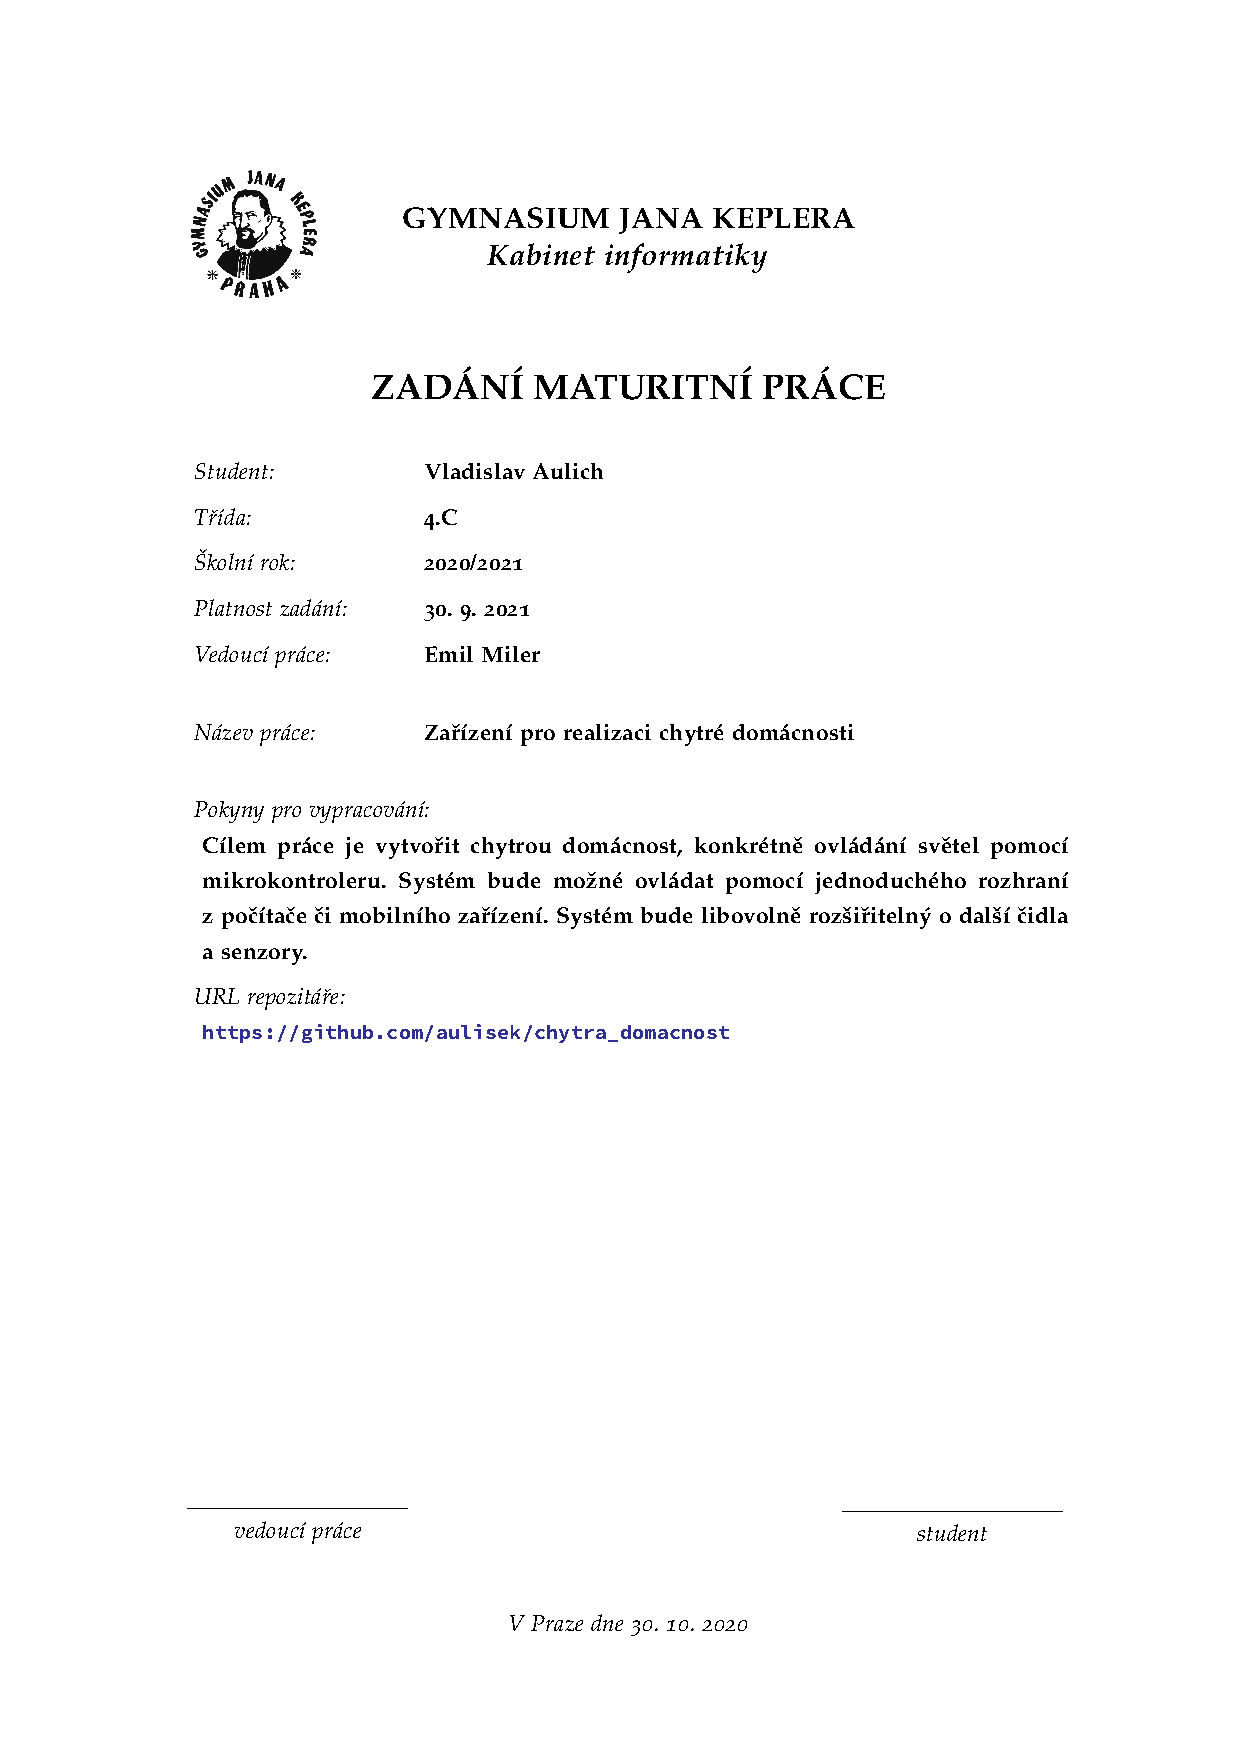
\includepdf[]{zadani.pdf}


%%% Strana s čestným prohlášením k bakalářské práci

\hypersetup{pageanchor=true}
\cleardoublepage
\vspace*{\fill}
\section*{Prohlášení}
\noindent
\Prohlaseni

\vspace{2cm}
\noindent
V Praze dne \today
\hspace*{\fill}\small{\AutorPrace}
\vspace{1cm}

%%% Poděkování
\openright
\vspace*{\fill}
\section*{Acknowledgement}
\noindent
\Podekovani
\vspace{1cm}


%%% Povinná informační strana bakalářské práce
\openright
\section*{Souhrn}
\noindent
\Abstrakt
\subsection*{Klíčová slova}
\noindent
\KlicovaSlova

\bigskip\bigskip\bigskip
\section*{Summary}
\noindent
\AbstraktEN
\subsection*{Keywords}
\noindent
\KlicovaSlovaEN

\openright
\pagenumbering{arabic}
	
	% Obsah
	\setcounter{tocdepth}{2}
	\tableofcontents
	
	\chapter{Introduction}
	\pagestyle{fancy}

	\section{Studied compounds}
    \subsection{Polylactic acid}

    \subsection{Active pharmaceutical ingredients}
    
   % \subsubsection{Ibuprofen}
    
    %\subsubsection{Naproxen}
    The second selected API is \textbf{naproxen} a non-steroidal anti-inflammatory drug, used as a painkiller. Naproxen contains three oxygen atoms (one carboxyl group and one ether bond), the structure is shown in Figure \ref{fig:APIs} on the right. According to its structure, naproxen can donate one hydrogen bond and accept up to three hydrogen bonds. Naproxen is a white crystalline powder, with a molar weight of $M_\mathrm{w}$~=~230.263~$\mathrm{g\ mol^{-1}}$ and melting point 429.3 K \cite{stejfa}. 
    
    %\subsubsection{Carbamazepine}
    \textbf{Carbamazepine} is a representative anticonvulsant, which is used for the treatment of seizures and neuropathic pain. Carbamazepine contains two nitrogen atoms (amide group) and one oxygen in the carboxyl group; its structure is shown in Figure \ref{fig:APIs} on the left side. According to its structure, carbamazepine can accept and donate one hydrogen bond. Carbamazepine is a white crystalline powder, with a molar weight of $M_\mathrm{w}$~=~236.273~$\mathrm{g\ mol^{-1}}$ and melting temperature of 463.6 K \cite{stejfa}.
    
    %\subsubsection{Indomethacine}
    
    %\subsubsection{Sulfathiazole}
    The selected API was \textbf{sulfathiazole} as a representative antibiotic drug from the sulfonamides group, which is used in the treatment of pyogenic cutaneous infections \cite{sulfathiazole_usage}. Sulfathiazole is a white crystalline powder, with molar weight $(M_\mathrm{w})$ =255.3 $\mathrm{gmol^{-1}}$ \cite{sulfathiazole}, which is highly polymorphic, there are 5 polymorphs discovered so far \cite{caron}. All known polymorphs of sulfathiazole crystallize in the $P2_1/c$ space group, but there are differences in intermolecular bonding and structural properties \cite{sulfathiazole_exp}. For our research, we chose the II polymorph, the structure of which is pictured in Figure \ref{fig:sulfathiazole}, there are four molecules of sulfathiazole in the crystal monoclinic unit cell. Our goal is to use quantum computing methods to determine the charges on atoms to complete the force field file model, and then to use MD to validate the model through comparison of simulated crystallographic parameters and density with experimental data.
    
    \begin{figure}[htb!]
        \begin{subfigure}{0.5\textwidth}
        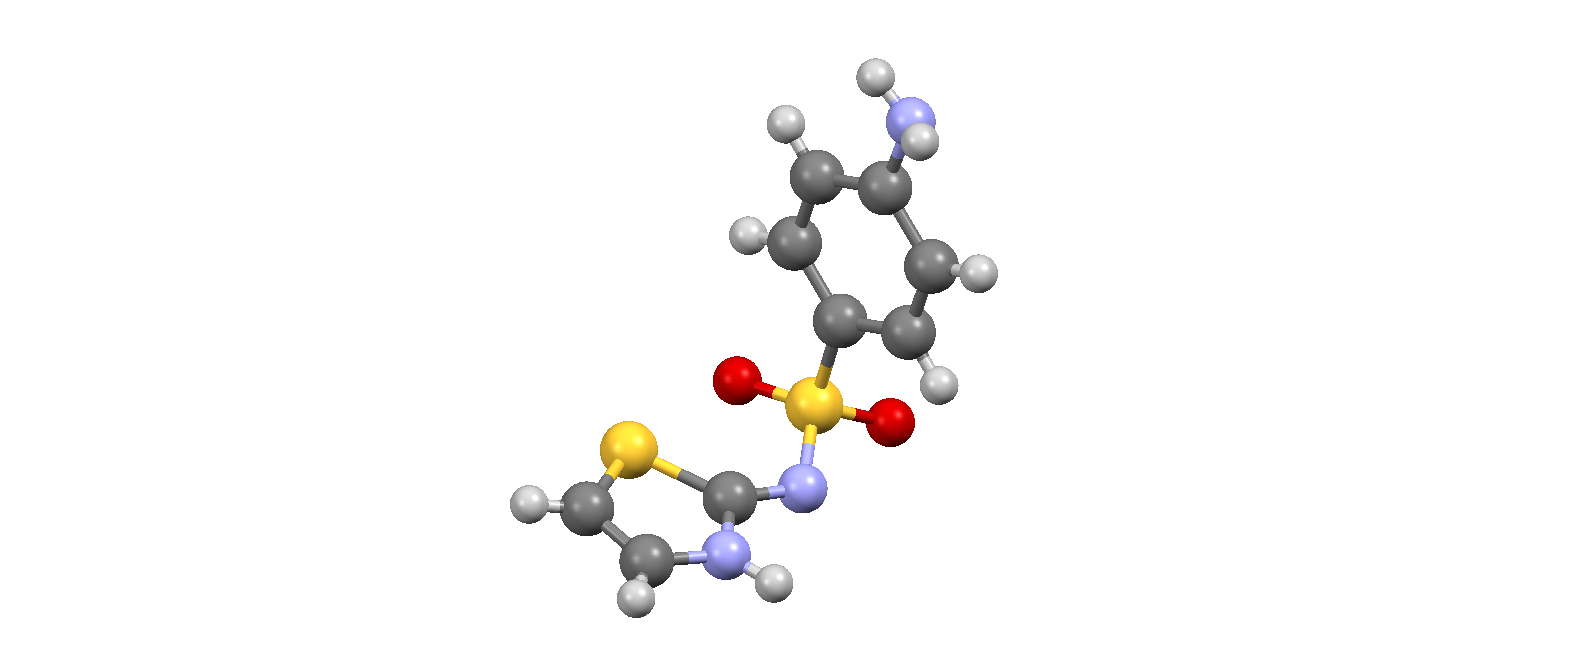
\includegraphics[1\linewidth]{img/sulfathiazol.png} 
        \end{subfigure}
        \begin{subfigure}{0.5\textwidth}
        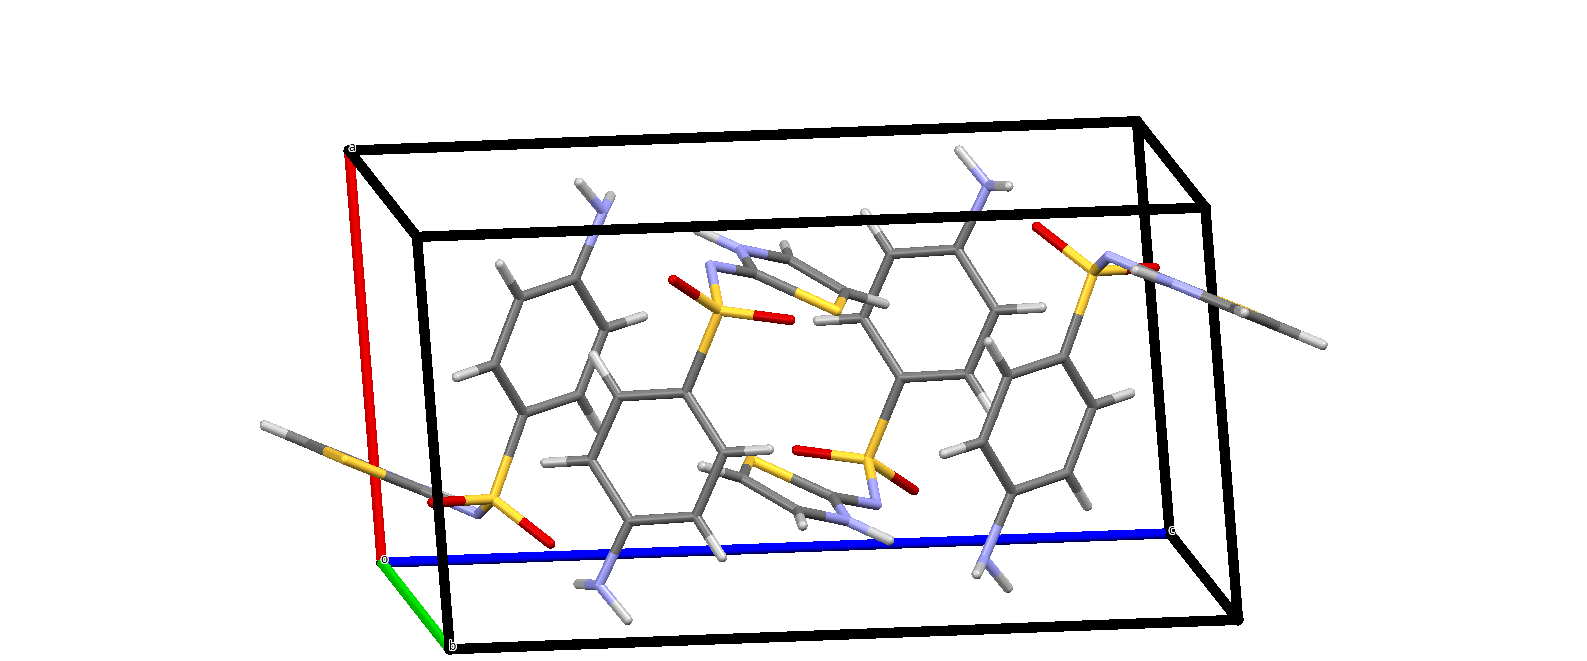
\includegraphics[1\linewidth]{img/sulfathiazol_packing.png}
        \end{subfigure}
        \caption{Sulfathiazole - molecular structure on the left and a unit cell of its II polymorph on the right.}
        \label{fig:sulfathiazole}
    \end{figure}
	

	\chapter{Theoretical part}

	
	\chapter{Computational methods}

    \chapter{Results and discussion}
	
	
	
	\chapter*{Conclusion}
	\pagestyle{empty}
	\addcontentsline{toc}{chapter}{Conclusion}
	
	
	%%% Seznam použité literatury
	\printbibliography[title={References},heading={bibintoc}]
	
	%%% Seznam obrázků
	\openright
	\listoffigures
	\addcontentsline{toc}{chapter}{Seznam obrázků}
	
	%%% Seznam tabulek
	\clearpage
	\listoftables
	\addcontentsline{toc}{chapter}{Seznam tabulek}
	
	%%% Přílohy k práci, existují-li. Každá příloha musí být alespoň jednou
	%%% odkazována z vlastního textu práce. Přílohy se číslují.
	
	%\part*{Přílohy}
	%\appendix
	
\end{document}
